\chapter[Results and Discussion]{Results and Discussion}{Results and Discussion}\label{CH5:R&D}

%\section{Introduction}
In this section, numerical and experimental findings will be discussed in detail. The numerical simulations are conducted with a fixed equivalence ratio of $\phi = 0.8$. On the other hand, the experimental results cover a range of equivalence ratios from $\phi = 0.5$ to $\phi = 0.8$. The experimental data includes global images, spatially and temporally averaged CH* data, pollutant emissions, the lean operational limit, and the correlation between emission data and CH* intensity data.

\section{\textbf{Numerical results}}
The steady state numerical simulations are carried out by  using commercial softwares ANSYS FLUENT for both the combustor configurations. In particular, both non-reacting and reacting cases were numerically investigated. The obtained numerical results can provides detailed 3-D flow features in terms of the evolution of flow fields, temperature distribution, and recirculation ratios in the combustor. 

\subsection{Flow field Characteristics}

\subsubsection{Non-Reacting case}
Figure \ref{NonVelCont} shows velocity field for the PVRF and SPRF combustor non-reacting cases. The inlet velocities is 32 m/s for air and 61 m/s for fuel for both the combustors. PVRF combustor shows higher exit velocity around 40 m/s compared to SPRF combustor (i.e., 20 m/s) due to two exit ports in the SPRF combustor.
In the SPRF combustor, due to symmetry on both sides of the jet, there is no visble deflection in the jet, while in the PVRF combustor, the jet deflects towards the left wall of the combustor (opposite to the exit port) due to the low pressure region and creates a peripheral vortex. The resultant stagnation points are marked with red circle where its location is deviated slightly towards left in the case of PVRF combustor. The visible impact of number of exhaust ports can be clearly seen as the higher velocity is observed in the case of PVRF with single exhaust port.
\begin{figure}[h!]
\begin{subfigure}[t]{1\textwidth}
    \centering
    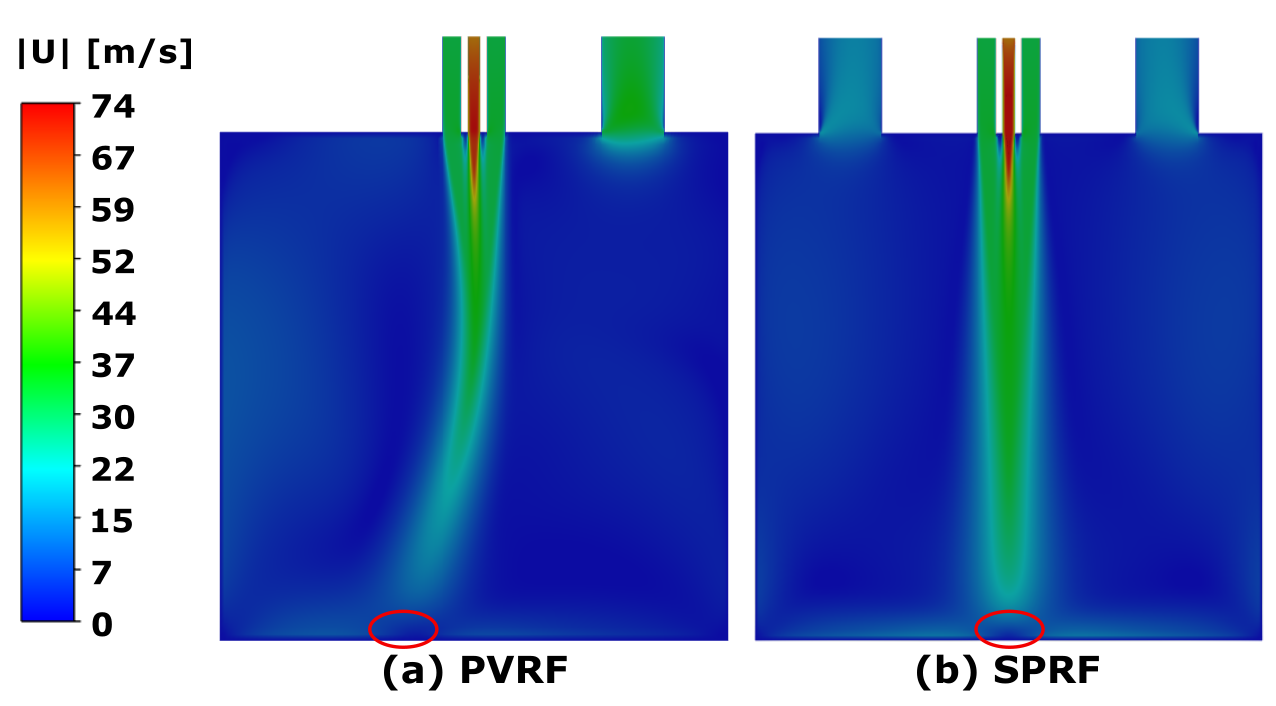
\includegraphics[width=0.7\textwidth]{Chapter5/Images/Numerical/Contours/vel_contsNonReacting.png}
    \subcaption{The mean velocity fields for non-reacting cases}
    \label{NonVelCont}
\end{subfigure}

 \begin{subfigure}[t]{1\textwidth}
	\centering
        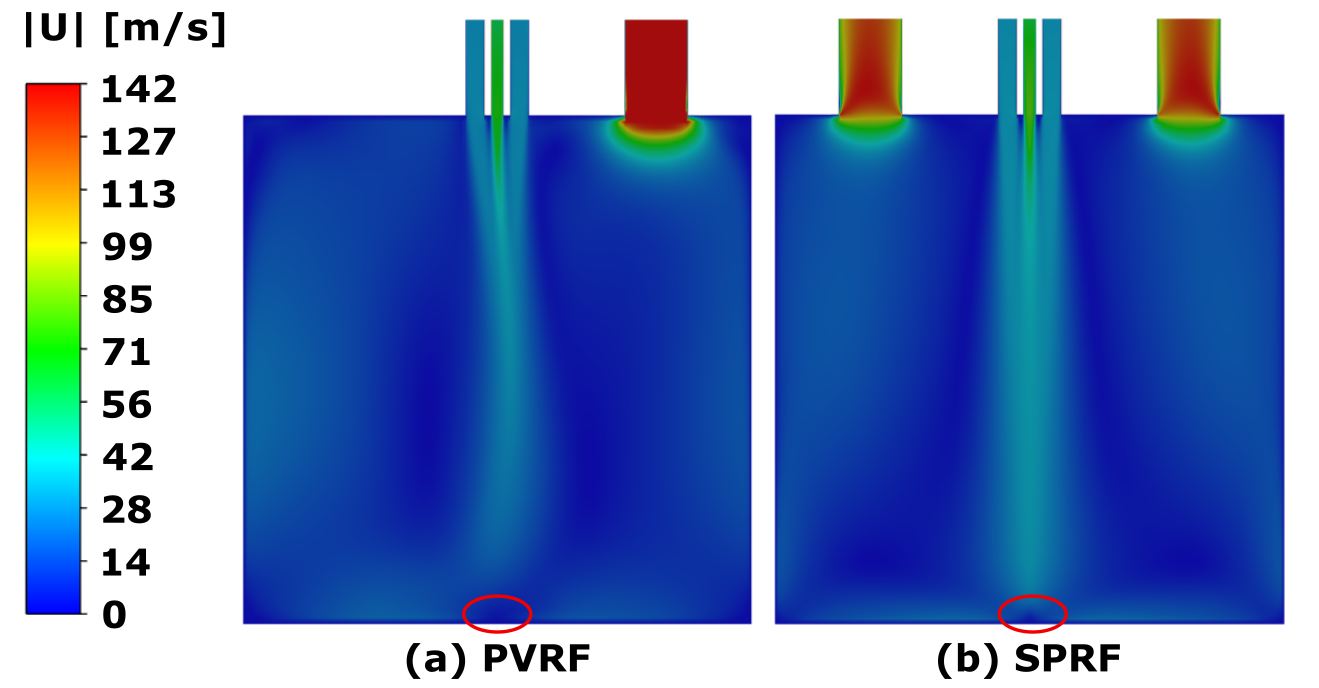
\includegraphics[width=0.73\textwidth]{Chapter5/Images/Numerical/Contours/vel_contsReacting.png}
	\subcaption{The mean velocity fields for reacting cases}
	\label{ReactingVelCont}
\end{subfigure}
\caption{Velocity Contours.}
\label{fig:FlowFieldContours}
\end{figure}

\subsubsection{Reacting case}

Velocity field for the reacting flow is shown in figure \ref{fig:FlowFieldContours} for both combustors. The air and fuel injection velocity are same as non-reacting cases. There is an overall increase in the velocity magnitude throughout the combustor as compared to the non-reacting cases because of temperature increment and decreased gas density. Again PVRF combustor shows higher exit velocity (240 m/s) than SPRF combustor (120 m/s). The resulting stagnation points for SPRF is still at the centre while, but relatively less deviated in the case of PVRF combustor as compared to non-reacting case. This observation can be attributed to complex flow dynamics and variation of thermo-physical properties of working fluid during combustion process. 

\subsection{Temperature field characteristics}
Figure \ref{TempContours} illustrates the temperature contours for both PVRF and SPRF combustors, with the temperature ranging from 300 to 2400 K. The fuel jet is surrounded by the air jet, and at the entry of the reactants, only air is present in the outer boundary of the jet. Due to the considerable recirculation of product gases, the reactions begin further downstream, where the fuel and air mix to form a reactive mixture. In the PVRF combustor, there is a distinct region of relatively lower temperature observed on right sides of the air jet, particularly in the central area of the combustor.

\begin{figure}[h!]
	\centering
        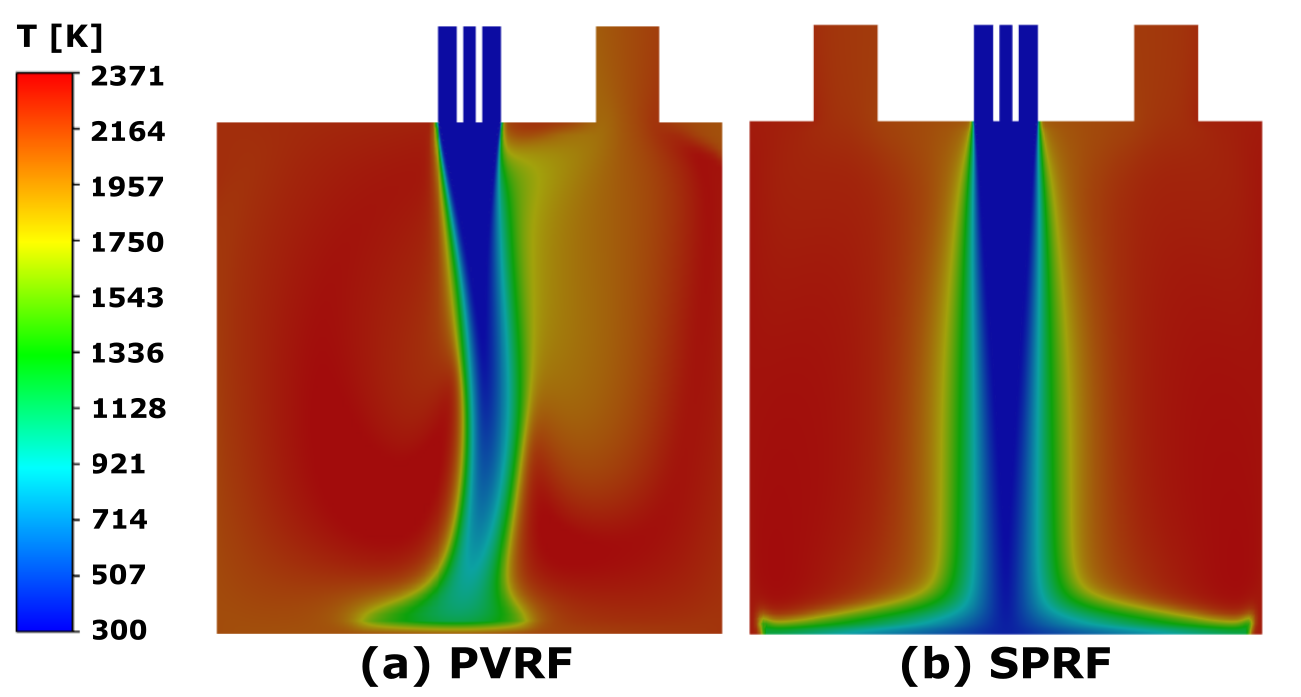
\includegraphics[width=0.7\textwidth]{Chapter5/Images/Numerical/Contours/temp_contsReacting.png}
	\caption{Temprature contours.}
	\label{TempContours}
\end{figure}

The rapid mixing facilitates the entrainment of hot flue gases into the reactants. Furthermore, in the SPRF combustor, a relatively more uniform temperature distribution is achieved. This is because of high momentum of the fuel jet and the presence of high-temperature regions surrounding the air jet. As a result, the combustion reaction primarily occurs at the center of the combustor, while the remaining combustion products are evenly distributed throughout the combustor. The bottom section of the combustor exhibits a near-uniform temperature, indicating the presence of a stagnation zone in that region.

\subsection{Recirculation ratio }

Recirculation ratios are calculated for both reacting and non-reacting conditions. To obtain the recirculation ratio, the entrained mass flow rate is divided by the mass flow rate of the injected fresh reactants, which includes both air and fuel.
\begin{align}
 Recirculation \ Ratio \ = \ \frac{\dot m_{recirc} - \dot m_{inj}}{\dot m_{inj}}
\end{align}
\subsubsection{Non-Reacting}
Figure \ref{NonRecirRatio} illustrates the evolution of the recirculation ratio of gases within the combustor along the length of the air jet as it progresses.
In non-reacting case (see Figure \ref{NonRecirRatio}), PVRF combustor recirculation ratio increases upto 5 y/D$_{air}$ (y is the combustor length in the jet axis) and then starts decreasing. In SPRF combustor recirculation ratio increases upto 4 y/D$_{air}$ and then decrease upto 5 y/D$_{air}$ then increases again up to 7 y/D$_{air}$ then decreases. The recirculation ratio magnitude for SPRF combustor is less than that for PVRF combustor. In both cases, the air jet diminishes as it reaches the bottom of the combustor, but the length of the combustor is not adequate for complete dissipation of the jet. Hence, the mixture reverses back mostly towards the right side as there is a wall present on the left side, which is closer to the jet core. From the right side, the gases rise up towards the exit. These gases tend to move out from the exit, but some gases move towards the incoming reactants. Recirculated gas entrainment increases the recirculation ratio linearly upto 5 y/D$_{air}$ and then decreases exponentially due to the presence of a stagnation zone at the lower portion of the combustor. It is important to note that a decrease in the recirculation ratio doesn’t imply there is no entrainment rather a weaker flow recirculation .
\begin{figure}[h!]
	\begin{subfigure}[t]{0.5\textwidth}
	    \centering
            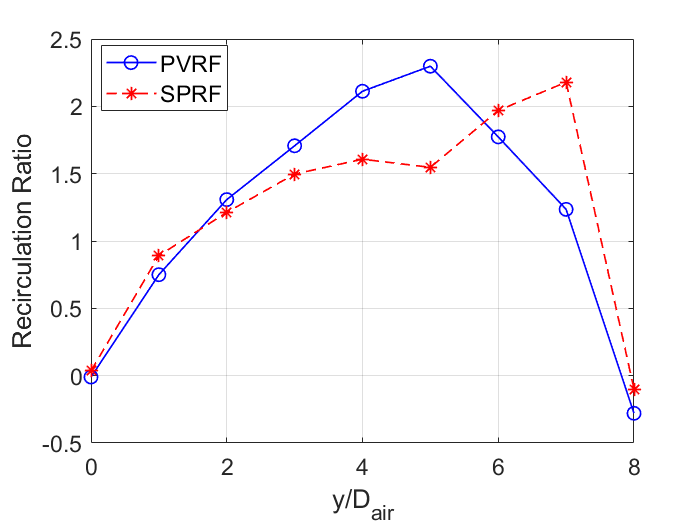
\includegraphics[width=0.95\textwidth]{Chapter5/Images/Numerical/Recirculation ratio/RR_NR.png}
    	\subcaption{Non reacting recirculation ratio}
    	\label{NonRecirRatio}
	\end{subfigure}
        \begin{subfigure}[t]{0.5\textwidth}
            \centering
            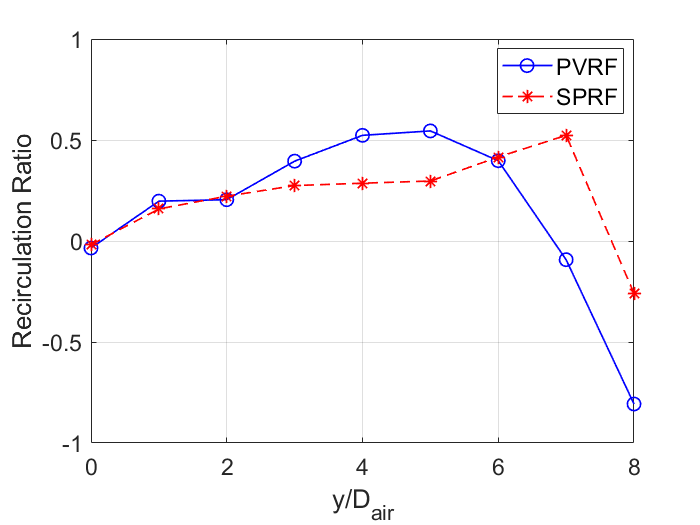
\includegraphics[width=0.95\textwidth]{Chapter5/Images/Numerical/Recirculation ratio/RR_R.png}
    	\subcaption{Reacting recirculation ratio}
    	\label{RecirRatio}
        \end{subfigure}
\caption{Recirculation Ratio.}
\label{fig:Recirculation Ratio}
\end{figure}

\subsubsection{Reacting}
In the case of the reacting flow (refer to Figure \ref{RecirRatio}), the recirculation ratio of the PVRF combustor initially increases until reaching a value of 5 y/D${air}$, after which it starts to decrease. On the other hand, the recirculation ratio of the SPRF combustor increases until a value of 7 y/D${air}$ and then decreases. SPRF combustor shows lower recirculation ratio than that of the PVRF combustor. Negative values indicate the existence of a stagnation region. It is noteworthy that the magnitude of the recirculation ratio in the reacting flow case is lower compared to the non-reacting cases. 

\section{Experimental Results}
In this section experimental results are discussed. Here CH* chemiluminescence data, global photographs and NOx and CO emissions levels at corrected to 15$\%$ O$_2$, lean operational limit and NOx and CH* intensity relationships are described.

\subsection{Global Imaging}
Global images are used for flame characteristics in the colorless combustion regime. These images, depicted in Figure \ref{global}, exhibit a faint bluish-violet coloration. This coloration suggests the presence of the CH* radical, which emits chemiluminescence at a wavelength of 432 nm. It is observed that the luminosity of these images diminishes as the equivalence ratio decreases.


\begin{figure}[h!]
	\centering
        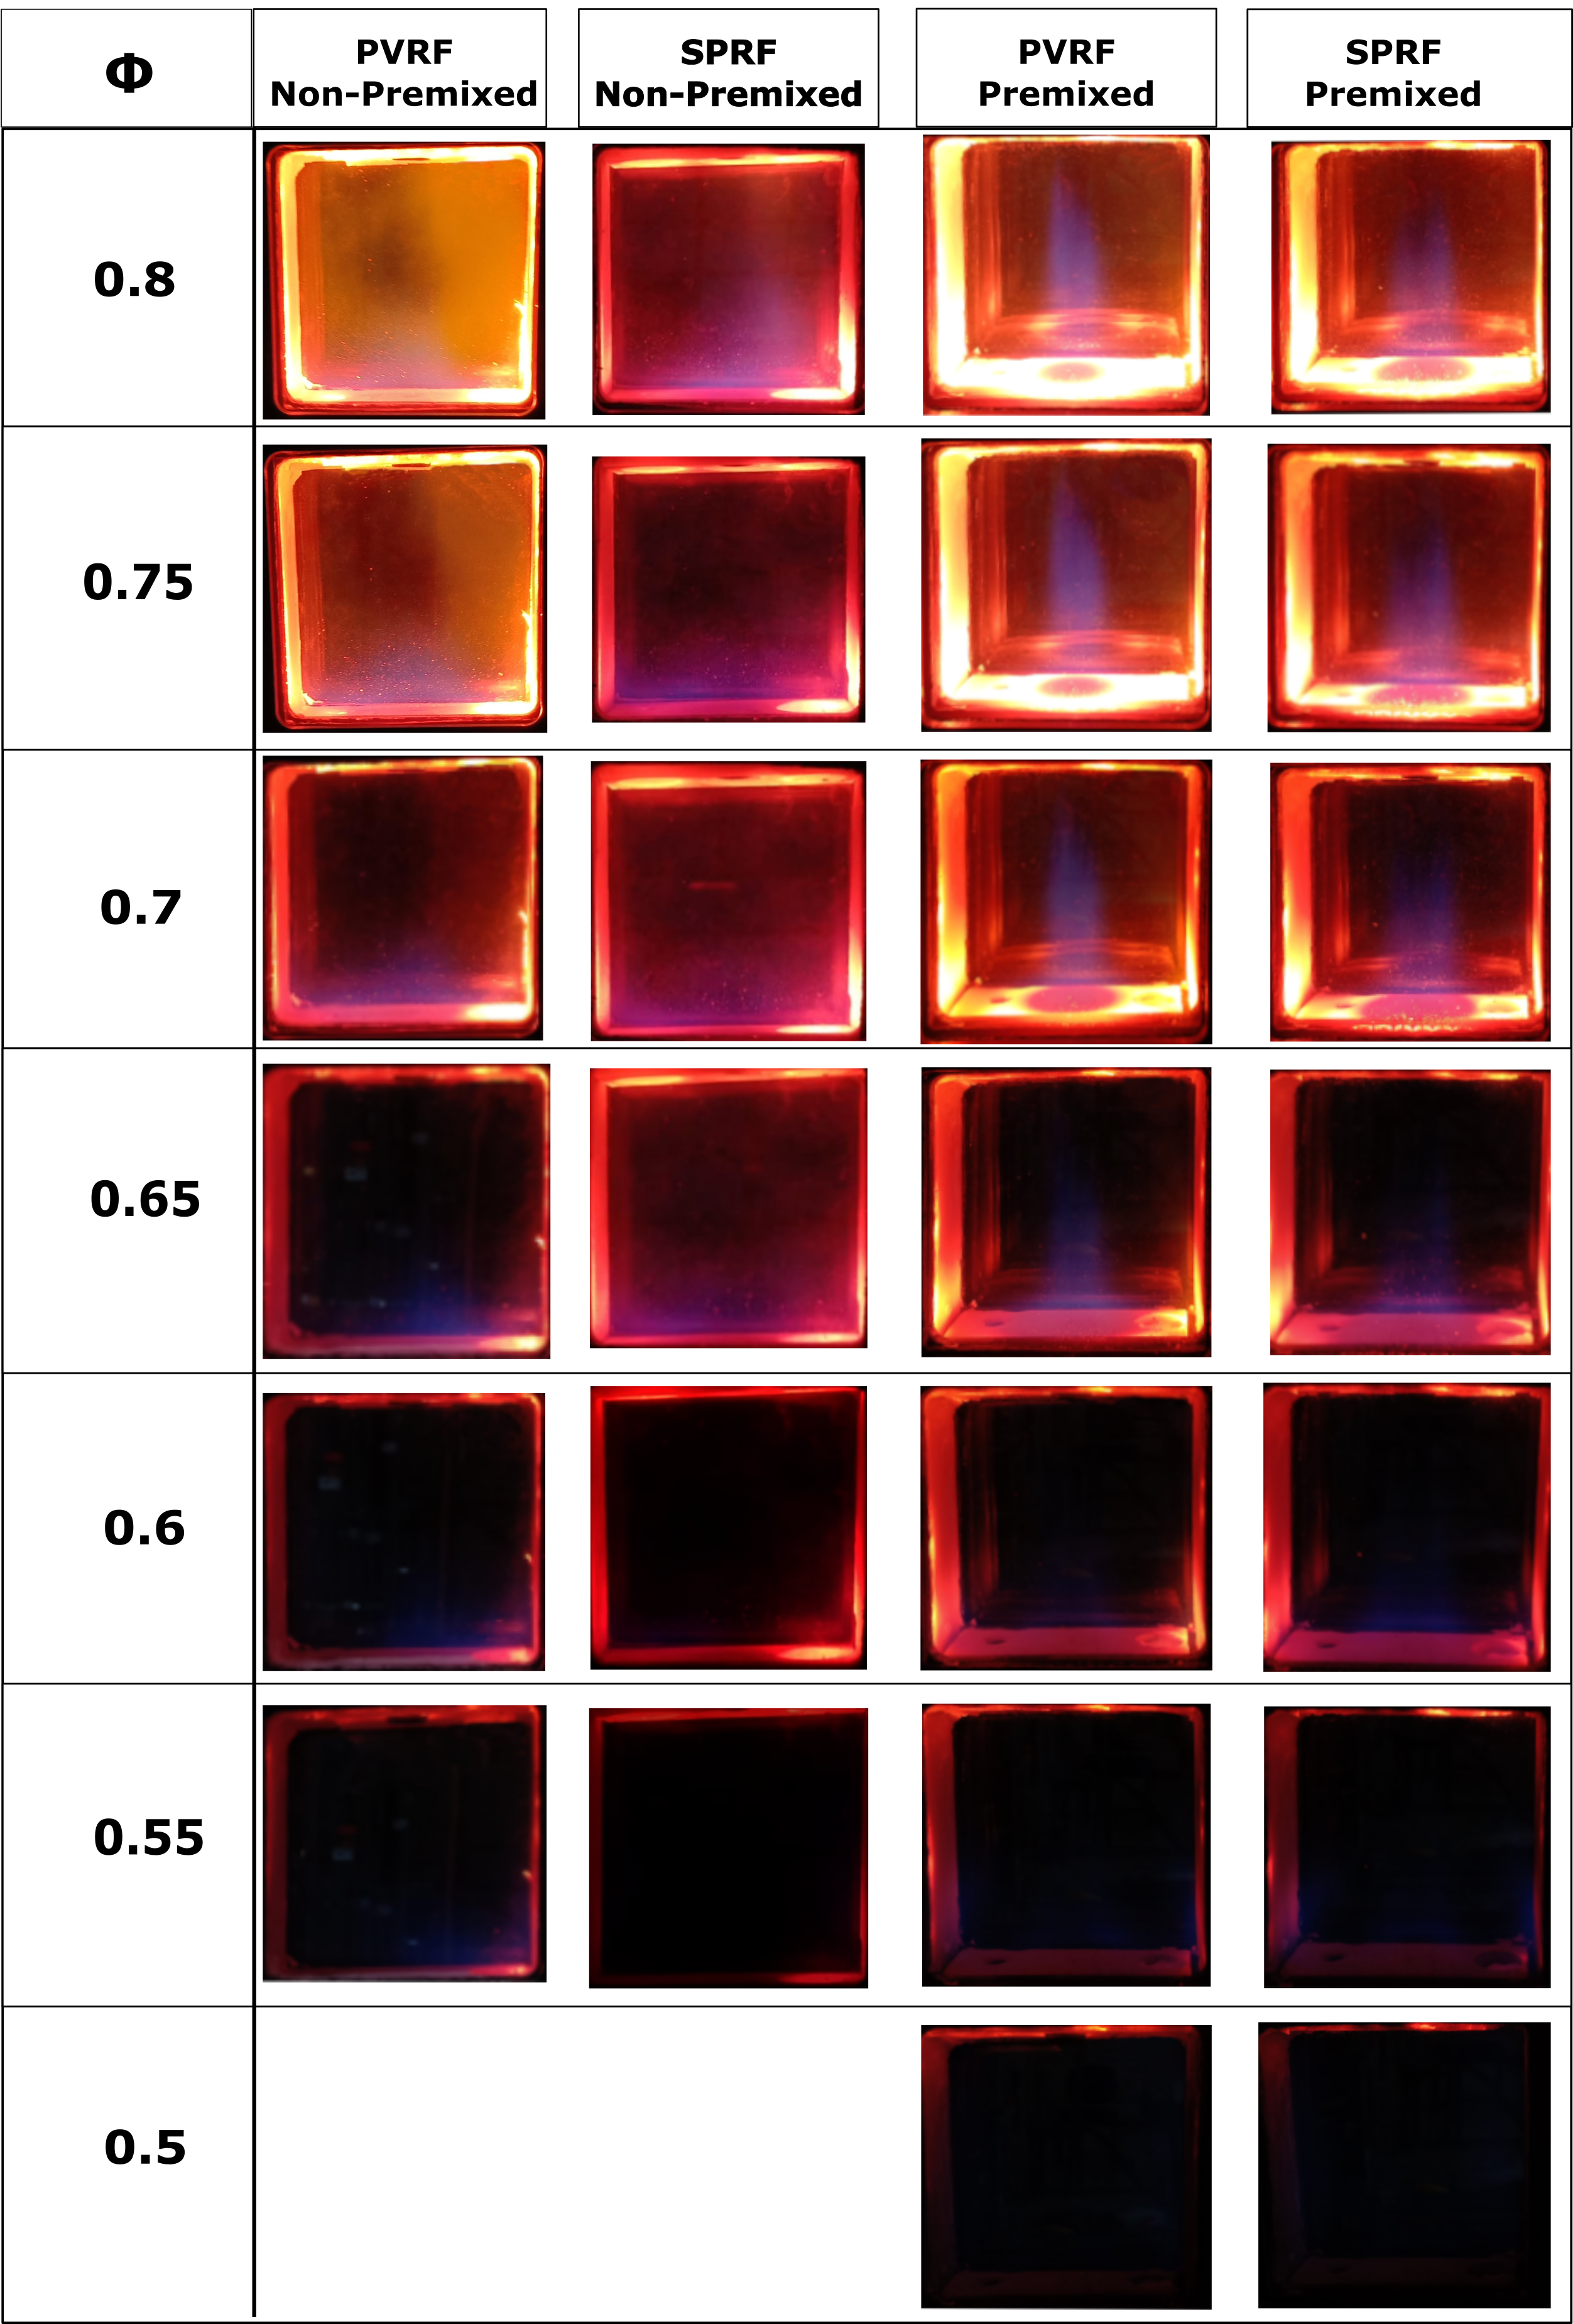
\includegraphics[width=0.95\textwidth]{Chapter5/Images/Experimental/Global images/Global.png}
	\caption{Global flame photographs of PVRF \& SPRF combustor}
	\label{global}

\end{figure}

\subsection{CH* chemiluminescence}
CH* chemiluminescence refers to the emission of light from chemical reactions. The intensity of chemiluminescence radiation in combustion process is influenced by the chemical kinetics \cite{AHMAD2023101200}. Reaction zone is identified using these characteristics.

\begin{figure}[h!]
	\centering
        \includegraphics[width=0.85\textwidth]{Chapter5/Images/Experimental/Chemiluminiscene/Chems.png}
	\caption{CH$^*$ chemiluminescence intensity images.}
	\label{SENP_chems}
\end{figure}

\begin{figure}[h!]
	\begin{subfigure}[t]{0.5\textwidth}
	    \centering
            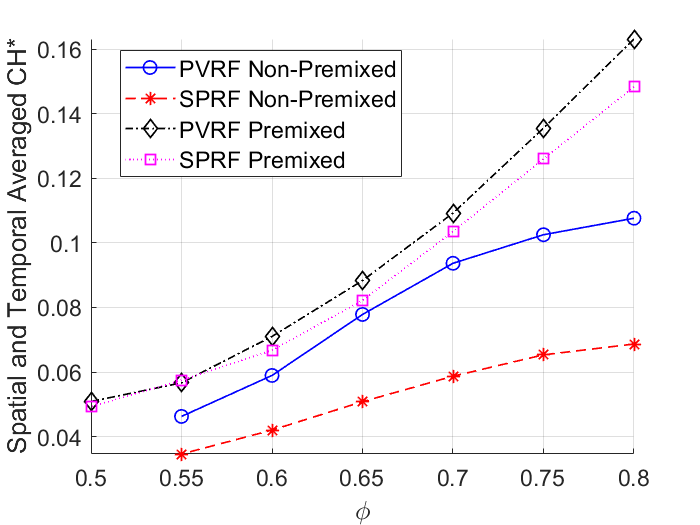
\includegraphics[width=0.95\textwidth]{Chapter5/Images/Experimental/Chemiluminiscene/imgAvgST1.png}
    	\subcaption{Averaged CH$^*$ intensity.}
    	\label{fig:AvgCHs}
	\end{subfigure}
        \begin{subfigure}[t]{0.5\textwidth}
            \centering
            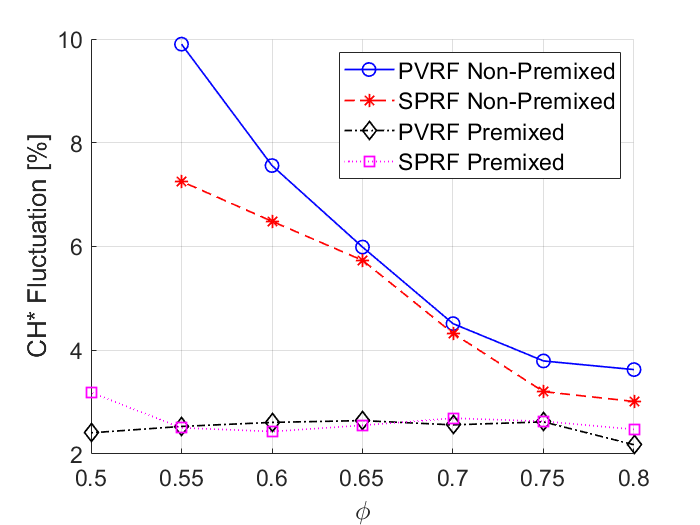
\includegraphics[width=0.95\textwidth]{Chapter5/Images/Experimental/Chemiluminiscene/coeffVar1.png}
    	\subcaption{ Averaged CH$^*$ coefficient of variation.}
    	\label{fig:CoeffVar}
        \end{subfigure}
\caption{CH$^*$ chemiluminesence data.}
\label{fig:ChemsData}
\end{figure}

In the non-premixed case of both PVRF and SPRF combustors, CH* radical concentration indicates reaction zone which is situated at the lower portion of the combustor. Intensity of this reaction zone decreases as the $\phi$ decreases. In premixed case, at higher $\phi$ the reaction zone is situated in the center of both PVRF and SPRF combustors. As $\phi$ decreases, reaction zone shifts towards the bottom of the combustor. This behavior is visible for both the combustors  as the equivalence ratio $\phi$ decreases, intensity of CH* decreases (see Figure~\ref{SENP_chems}).

Figure \ref{fig:ChemsData} illustrates the spatial and temporal averaged intensity of CH$^*$ in the combustion process. In general, premixed cases exhibit higher CH$^*$ intensity compared to non-premixed cases. Specifically, in the non-premixed case, the PVRF combustor displays higher CH$^*$ intensity compared to the SPRF combustor. However, in the premixed cases, similar CH$^*$ intensities are observed between the two combustors. It is important to note that as the $\phi$ increases, the CH$^*$ intensity also increases in both combustors. This can be attributed to the higher temperatures associated with higher $\phi$. Figure \ref{fig:CoeffVar} shows the coefficient of variation of spatially averaged CH$^*$ intensity. The figure demonstrates that the fluctuation in total heat release is higher in the non-premixed case compared to premixed case. Fluctuations decreases as the global $\phi$ increases, for both the PVRF and SPRF combustors, SPRF combustor exhibits lower fluctuations in comparison to the PVRF combustor.

\subsection{Emissions characteristics}
CO and $NO_x$ emissions measurements (corrected to 15$\%$ of $O_2$ concentration) are presented in this section. 
\subsubsection{CO Emissions}
CO emissions are shown for all four cases in figure \ref{Co Emissions}. For non-premixed case, CO emissions are higher at high equivalence ratios and gradually decreases till $\phi = 0.7$ upto 32 ppm for PVRF and 24 for SPRF combustor, and then increases. From figure \ref{Co Emissions} it is clear that CO emissions in SPRF combustor is lower than PVRF combustor for non-premixed case. For premixed case, CO emissions decreases upto $\phi=0.55$ upto 21 ppm for PVRF and 13 ppm for SPRF combustor and then there is sudden jump in emission. Again CO emissions is lower in SPRF combustor than PVRF in premixed case. At lower equivalence ratios, the temperature field is reduced, leading to a lower conversion rate of CO to $CO_2$. As a result, the levels of CO emissions increase in these conditions. One observation can be made that till $\phi=0.65$ CO emissions are high in non-premixed case than premixed after that premixed case showed higher CO emissions than non-premixed case at higher equivalence ratios.
\begin{figure}[h!]
    \begin{subfigure}[t]{0.5\textwidth}
        \centering
	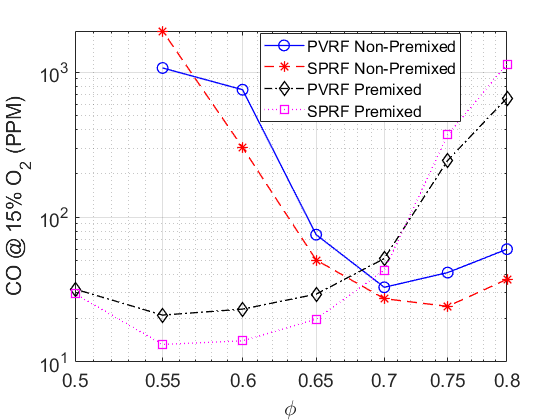
\includegraphics[width=0.95\textwidth]{Chapter5/Images/Experimental/Emissions/CO Emission.png}
	\subcaption{CO emission @ $15\%$ O$_2$}
	\label{Co Emissions}
    \end{subfigure}
    \begin{subfigure}[t]{0.5\textwidth}
        \centering
	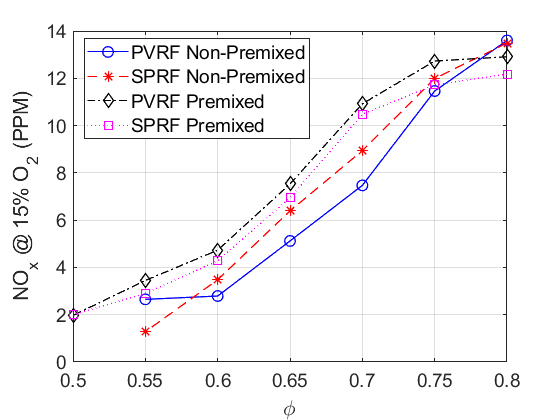
\includegraphics[width=0.95\textwidth]{Chapter5/Images/Experimental/Emissions/NoxEmmision.png}
	\subcaption{$NO_x$ emission @ $15\%$ O$_2$}
	\label{Nox Emissions}
    \end{subfigure}
\caption{CO and NOx Emissions.}
\label{fig:pollutantEmissions}
\end{figure}

\subsubsection{$NO_x$ Emissions }
$NO_x$ emissions are shown for all four cases in figure \ref{Nox Emissions}. For all cases, the maximum $NO_x$ emissions remain below 15 ppm when the equivalence ratio varies from 0.5 to 0.8 in the premixed case and 0.55 to 0.8 for non-premixed case. PVRF combustor in non-premixed case exhibits the lowest $NO_x$ emissions across the entire range of equivalence ratios. This is primarily attributed to the uniform and lower temperature distribution throughout the combustor, as well as improved fuel-oxidizer mixing. SPRF combustor shows higher $NO_x$ emissions than PVRF combustor. These $NO_x$ emissions are different from the generic $NO_x$ distribution at high equivalence ratios due to high CO emissions. 

\subsubsection{NO$_x$ and CH$^*$ intensity} Figure \ref{fig:NoxVsCo CHs} shows the correlation between NO$_x$ emissions and the spatially and temporally averaged CH$^*$ intensity. The graph illustrates a strong relationship between these two variables, particularly in the premixed case. It suggests that NO$_x$ emissions can be effectively estimated using CH$^*$ data, highlighting the potential for utilizing CH$^*$ measurements as an indicator of NO$_x$ emissions, especially in premixed mode.

\subsubsection{Lean Operational Limit}
Lean operational limit is determined by gradually decreasing the $\dot{m}_{fuel}$ while keeping the $\dot{m}_{air}$ constant until the flame extinguishes. The outcomes of this investigation are illustrated in Figure \ref{fig:LOL}. It can be observed that for both the PVRF and SPRF combustors, the lean limit is 0.5 for the premixed mode and 0.55 for the non-premixed mode.
\begin{figure}[t]
    \begin{subfigure}[t]{0.5\textwidth}
        \centering
	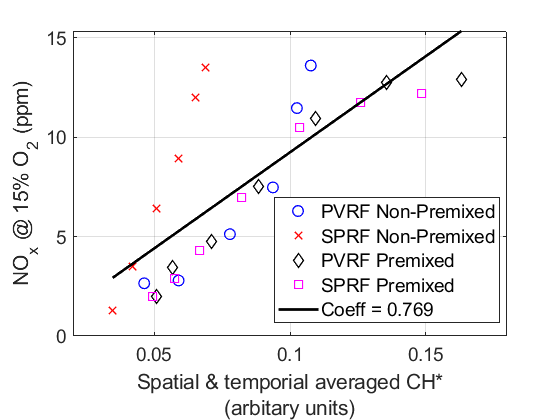
\includegraphics[width=0.95\textwidth]{Chapter5/Images/Experimental/Emissions/NOxVsCHs.png}
	\subcaption{NO$_x$ vs. CH$^*$ chemiluminescence intensity.}
	\label{fig:NoxVsCo CHs}
    \end{subfigure}
    \begin{subfigure}[t]{0.5\textwidth}
        \centering
	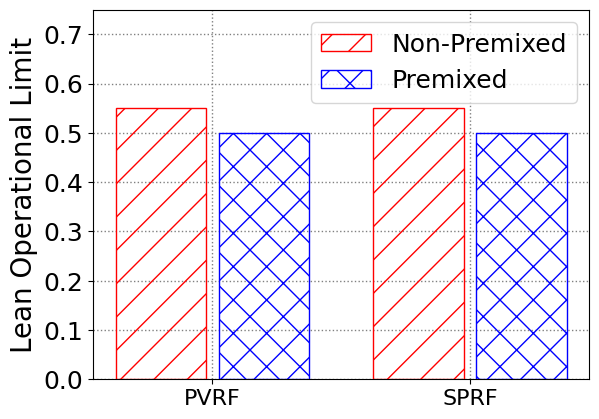
\includegraphics[width=0.95\textwidth]{Chapter5/Images/Experimental/Emissions/LoL.png}
	\subcaption{Lean operational limit.}
	\label{fig:LOL}
    \end{subfigure}
\caption{Nox vs CH$^*$ intensity and lean operational limit.}
\label{fig:NOxChsansLOL}
\end{figure}